\begin{figure*}[!tb]
\paperfigure{figures/anchor_framework.pdf}{fig:framework}{Schematic AnchorMTM workflow: extraction and referencing, topology-budgeted layout, and topology-to-1D reconstruction produce the temporal map. The layout panel combines leaf-order search and anchor placement.}
\end{figure*}
\section{AnchorMTM}\label{sec:method}\label{sec:construction}

Figure~\ref{fig:framework} summarizes the construction; its topology-budgeted layout panel contains the separate order-search and anchor-placement stages. Extract and Reference prepares the trees, identities and fixed targets defined in Section~\ref{sec:formulation}. Search Leaf Orders chooses an admissible order with low $\tau$. Place Anchors balances spatial and temporal objectives within a cap on that order's displacement. Reconstruct and Assemble builds the scalar profiles and stacks them along time. The output of each stage fixes the constraints passed to the next. The control is a normalized merge allowance $\varepsilon$, with $\eta=(\varepsilon_0+\varepsilon)\Delta_F$ for sequence scalar range $\Delta_F$ and numerical tolerance $\varepsilon_0=10^{-7}$. Exact Mode sets $\varepsilon=0$; the exact experiments use zero labelled error. Budgeted Mode uses a positive allowance within the same construction. Balanced denotes an experimentally selected positive-budget configuration, not all budgeted maps. Widths, gap, slack and weights stay fixed during a budget sweep; the merge allowance controls hierarchical error rather than directly bounding positional error.

\subsection{Order Selection and Optimal Barriers}
Order search receives the prepared tree, reference targets, widths and merge allowance. A finite candidate pool $\mathcal C$ starts from midpoint orders of the strict tree, threshold flattenings and selective conflict flattenings. Width-aware block moves refine promising structures. The point bound supplies an exact-topology initialization, while the interval analysis motivates evaluating packing displacement. Each visited order is checked against the original merge matrix, and selection is lexicographic:
\begin{equation}\label{eq:orderobjective}
\pi^\varepsilon\in\arg\min_{\pi\in\mathcal C}\bigl(\tau(\pi),\nroe(\pi)\bigr)
\quad\mathrm{s.t.}\quad\delta^*(\pi)\le\eta.
\end{equation}
The exact tree supplies a feasible strict-topology seed. Selective flattening releases additional permutations while retaining deeper blocks, as illustrated in Fig.~\ref{fig:selective_relaxation}.

\paragraph{Construction sequence.} For each frame, generate and refine candidate orders; compute $\tau$, NROE and $\delta^*$; admit the budget-feasible orders; choose the lexicographic minimum; solve its capped QP; fill and correct the profile; then check the rendered merge matrix and append the temporal column. The supplementary algorithm lists these steps with the tracking and rounding procedures.

\begin{figure}[!tb]
\centering
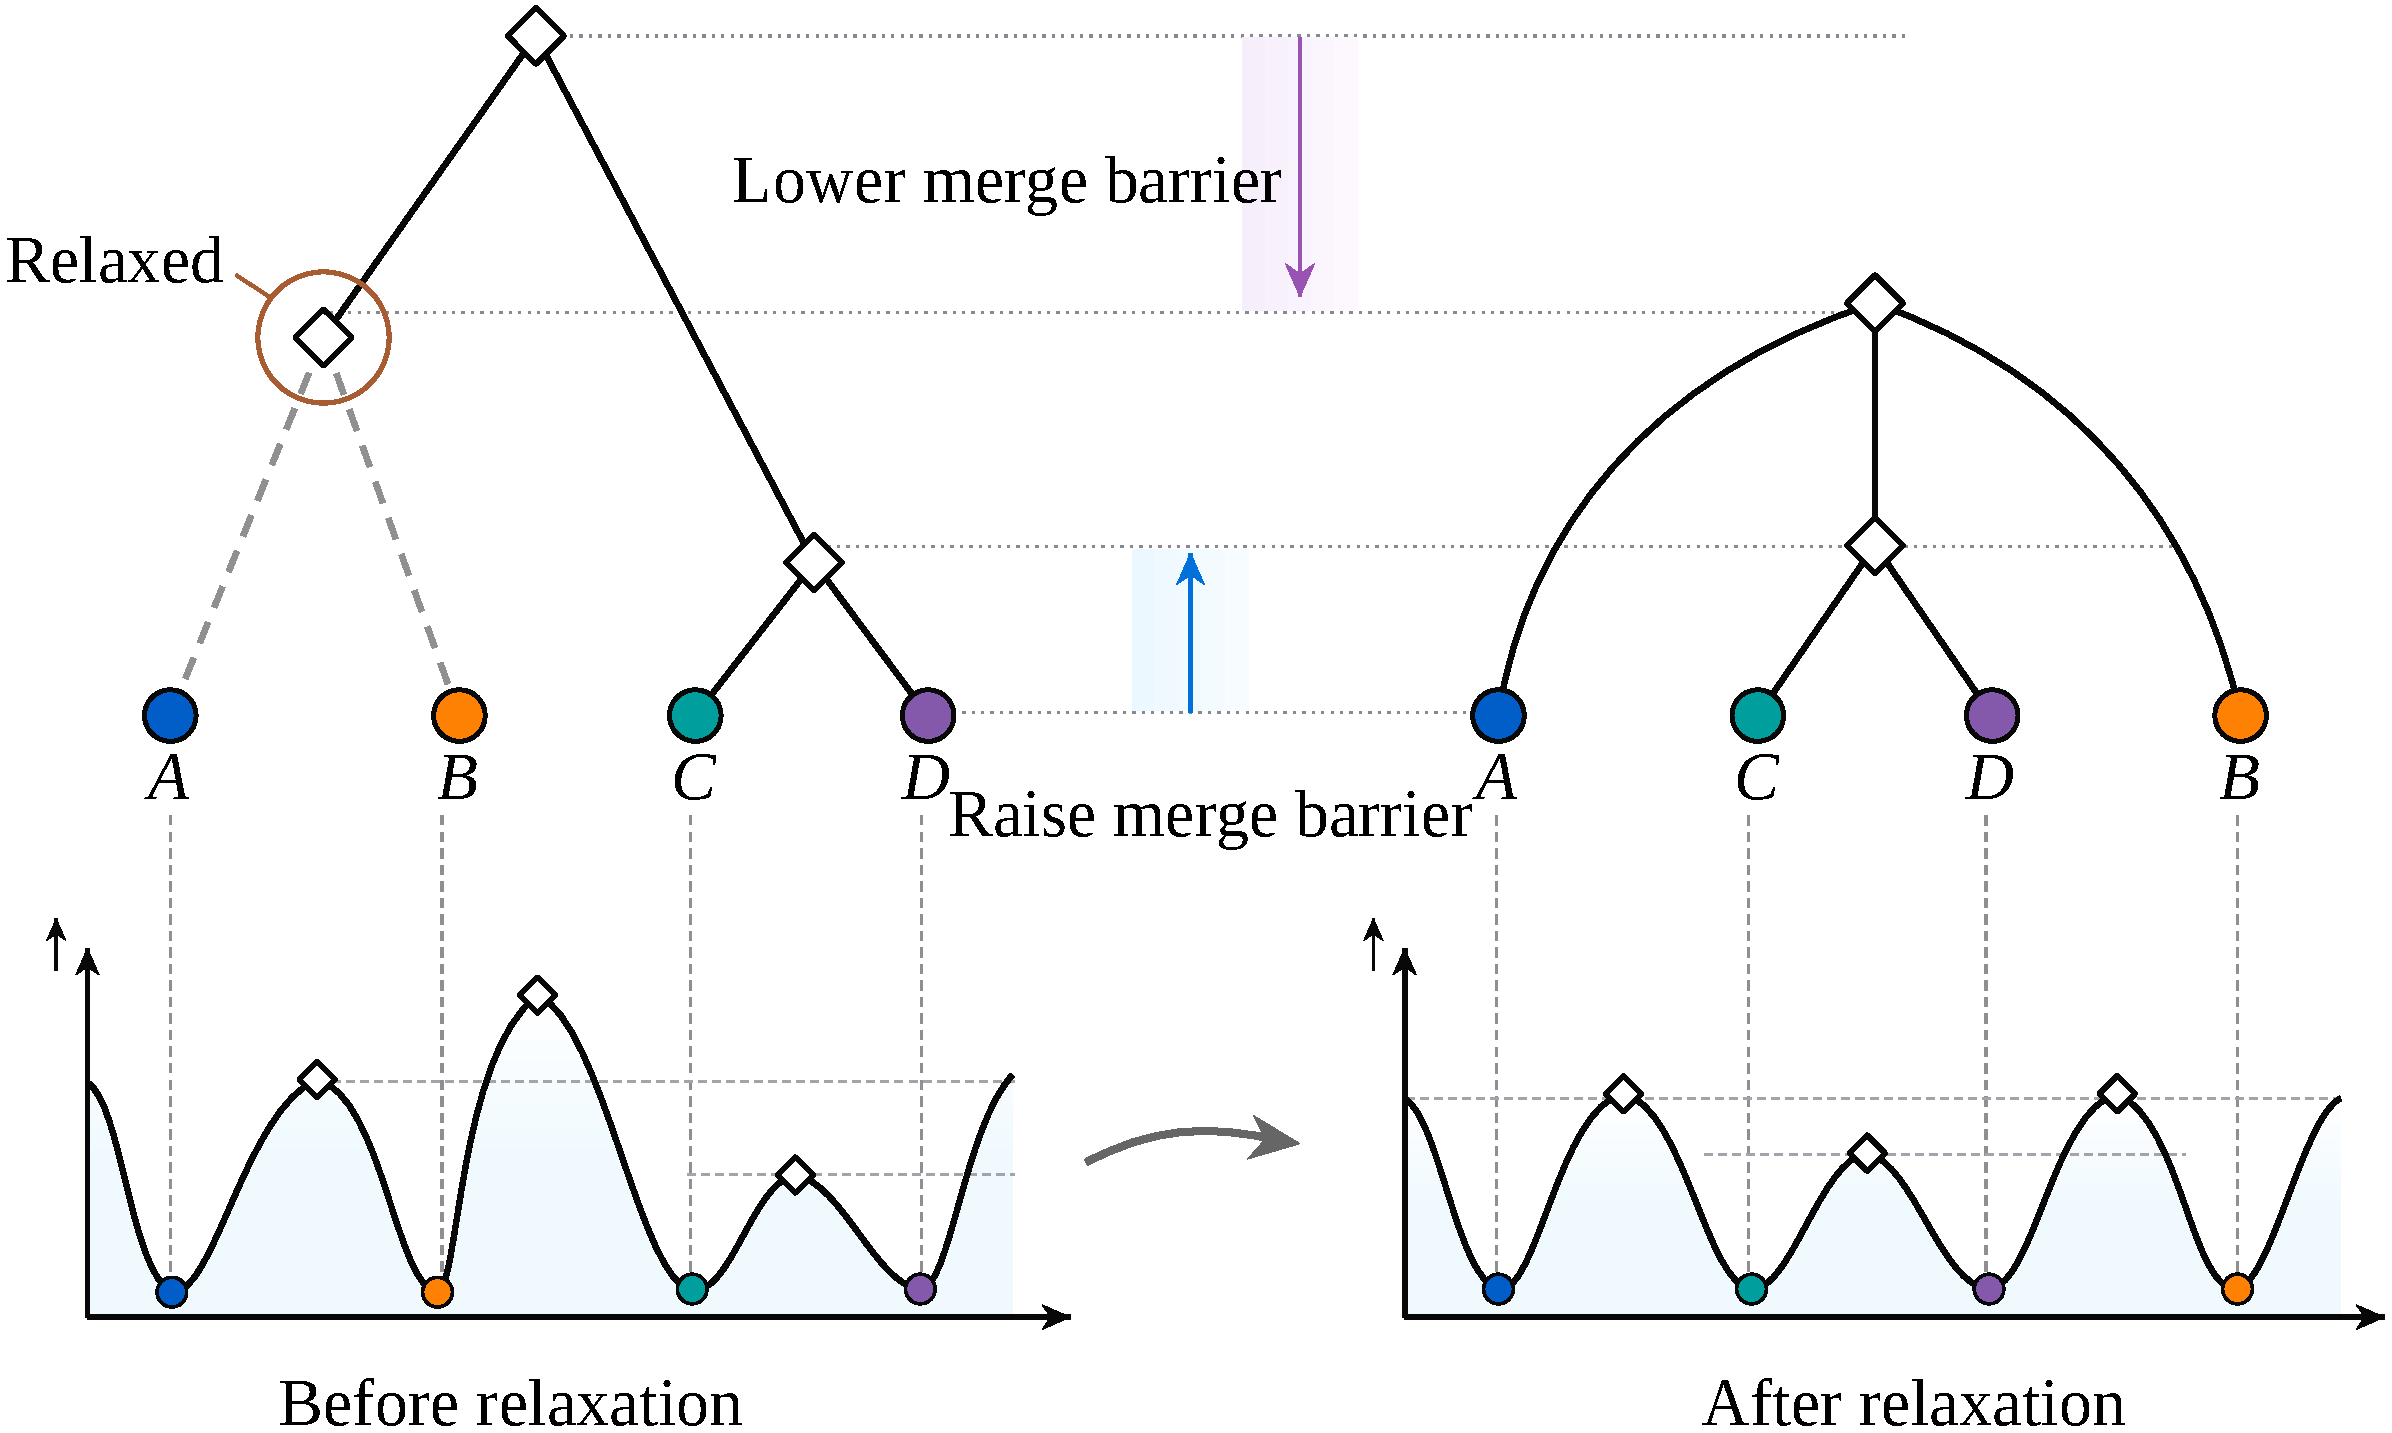
\includegraphics[width=\columnwidth]{figures/anchor_relaxation_open.pdf}
\caption{Selective flattening admits order $A,C,D,B$ while retaining the $C,D$ grouping. The displayed barrier levels are corrected against the original merge matrix.}
\label{fig:selective_relaxation}
\end{figure}
For gap $k$ of an order, set $C_k=\min_{i\le k<j}V_{\pi(i)\pi(j)}$ and let $F_k$ be the larger adjacent extremum value.
\begin{proposition}[Optimal barriers]\label{prop:barriers}
With fixed extrema, the least continuous merge error is
\begin{equation}\label{eq:delta}
\delta^*(\pi)=\max\Bigl\{0,\max_k(F_k-C_k),
\tfrac12\max_{i<j}\bigl(V_{\pi(i)\pi(j)}-\max_{i\le k<j}C_k\bigr)\Bigr\},
\end{equation}
attained by $b_k=C_k+\delta^*(\pi)$.
\end{proposition}
Indeed, error $\delta$ requires $F_k\le b_k\le C_k+\delta$; choosing the largest permitted barriers meets every pair's lower requirement exactly when $\delta\ge\delta^*$. This gives a closed-form admission test for candidate orders.

\subsection{Capped Spatiotemporal Placement}
For the chosen order, the default weights are $(\lambda_R,\lambda_G,\lambda_M,\lambda_C)=(4,1,0.5,0.1)$. Each term in Eq.~\ref{eq:family} is a mean squared residual: anchor-to-reference distance, ordered anchor separation minus support-centroid distance, matched temporal-target error, or anchor-to-center offset. The temporal target follows projected motion:
\begin{equation}\label{eq:temporal_target}
\hat x_i^t=x_{\mu_t(i)}^{t-1}+q_i^t-q_{\mu_t(i)}^{t-1}.
\end{equation}
The selected order is now fixed, so placement changes coordinates without revisiting the discrete search. Unmatched leaves have no temporal penalty. Placement solves the convex quadratic objective under the interval constraints and
\begin{equation}\label{eq:qp}
\|x-q\|_\infty\le\tau(\pi^\varepsilon)+\beta_0,
\end{equation}
with fixed slack $\beta_0$. Because $\tau$ is attained, this cap is feasible and transfers the selected order's displacement control to the final anchors. The cap prevents a relative-distance or temporal term from moving an anchor arbitrarily far from its spatial target. Conversely, the fixed slack leaves room to improve these secondary relationships after the discrete order has been chosen. Within a frame the feasible set is linear and the objective quadratic; frame order enters only through matched predecessor targets.

\subsection{Profile Reconstruction}
The final stage receives the order, anchor intervals and optimal barriers. Leaf-arc samples fill the intervals and LCA paths fill their gaps~\cite{Koepp:2023:TMTM,STMTM:2026}. Barrier correction clips each inter-anchor interior to $b_k$ and raises its peak when needed. Profiles share direction, origin, extent and pixel scale; their stack is $I^\varepsilon(t,u)=\psi_t^\varepsilon(u)$. Integer rounding can affect merge levels, so the rendered fixed-label matrix, including its diagonal, is checked after reconstruction. The supplementary material supplies the full algorithm and rounding procedure.
